\documentclass[twoside]{amsart}
\usepackage{amssymb,latexsym}
\usepackage{amsfonts}
\usepackage{xspace}
\usepackage{enumerate}
\usepackage{graphics}
\usepackage{fitch}
\newcommand{\Rationals}{\mathbb{Q}{}}
\newcommand{\Reals}{\mathbb{R}{}}
\newcommand{\Integers}{\mathbb{Z}{}}
\newcommand{\solution}{\textsc{Solution}\xspace}
\newcommand{\problem}{\textsc{Problem}\xspace}
\newcommand{\Blank}{\mathrel{\phantom{=}}}
\newcommand{\ltrue}{\top}
\newcommand{\lfalse}{\bot}
\newcommand{\fOfg}{\ensuremath{f \circ g}\xspace}
\newcommand{\gOff}{\ensuremath{g \circ f}\xspace}
\begin{document}
\title{Answers to Chapter 6 Exercises - A Book of Abstract Algebra}
\author{Michael Welch}
\date{\today}
\maketitle

This document contains selected answers to exercises from chapter 6
of A Book of Abstract Algebra.


\begin{enumerate}[A.]
   \item \textsc{Examples of Injective and Surjective Functions}

   \noindent Each of the folowing is a function $f:\mathbf{R}\to\mathbf{R}$.
   Determine
   \begin{enumerate}[(a)]
      \item whether or not $f$ is injective, and
      \item whether or not $f$ is surjective.
   \end{enumerate}
   \noindent Prove your answer in either case.

   \noindent \textbf{Example 1}

   \noindent 1. $f(x)=3x+4$

   \noindent $f$ is injective
   \begin{proof}
   Suppose $f(a)=f(b)$, that is, 
   \begin{align*}
       3a+4&=3b+4\\
       3a&=3b\\
       a&=b \qedhere
   \end{align*}
   \end{proof}

   \noindent $f$ is surjective. 
   \begin{proof}
   Take any element $y\in\mathbb{R}$. Then $y=3((y-4)/3) + 4=f((y-4)/3)$.
   Thus, every $y\in\mathbb{R}$ is equal to $f(x)$ for $x=(y-4)/3$.
   \end{proof}

   \noindent 2.  $f(x)=x^3+1$

   \noindent $f$ is injective.
   \begin{proof}
      Suppose $f(a)=f(b)$, that is,
      \begin{align*}
         a^3+1 &= b^3+1 \\
	 a^3   &= b^3   \\
	 \sqrt[3]{a^3} &= \sqrt[3]{b^3}\\
	 a &= b \qedhere
      \end{align*}
   \end{proof}

   \noindent $f$ is surjective.
   \begin{proof}
   Take any element $y\in\mathbb{R}$. Then $y=(\sqrt[3]{y-1})^3 + 1 =
   f(\sqrt[3]{y-1})$.
   Thus, every $y\in\mathbb{R}$ is equal to $f(x)$ for $x=\sqrt[3]{y-1}$.
   \end{proof}

   \noindent 3. $f(x)=|x|$
   
   \noindent $f$ is not injective. $f(3)=f(-3)=3$ yet $3\ne -3$.

   \noindent $f$ is not surjective. There is no value of $x$
   for which $f(x)=-3$.

   \noindent 4. $f(x)=x^3-3x$

   \noindent $f$ is not injective. $f(0)=f(\sqrt{3})=f(-\sqrt{3})=0$ yet
   $3\ne-3$.

   \noindent $f$ is surjective. It is continuous function and unbounded.

   \noindent 5. $f(x) = \displaystyle 
      \begin{cases}
         \phantom{2}x &\text{if $x$ is rational}\\
	           2x &\text{if $x$ is irrational}
      \end{cases}$


   \noindent $f$ is injective
   \begin{proof}
      It must be stated that $f(x)$ is rational iff $x$ is rational
      and $f(x)$ is irrational iff $x$ is irrational (because $2x$
      is irrational if $x$ is irrational).

      Suppose $f(a)=f(b)$. Assume $f(a)$ is rational. Then $f(b)$
      is rational. Then by defintion of $f(x)$, $a=b$. Now, assume
      $f(a)=f(b)$ is irrational. Then $2a=2b$ and $a=b$.
   \end{proof}

   \noindent $f$ is surjective.
   \begin{proof}
   There are two cases to consider: $y$ is rational, and $y$ is irrational.
   \begin{enumerate}[(1)]
      \item Take any rational element $y \in \mathbb{R}$. Then every
      rational $y$ is
      equal to $f(x)$ for $x=y$.

      \item Take any irrational element $y \in \mathbb{R}$. Then $y=2(y/2)=
      f(y/2)$. Thus, every irrational $y$ is equal to $f(x)$ for 
      $x=y/2$.
   \end{enumerate}
   Therefore $f$ is surjective.
   \end{proof}

   \noindent 6. $f(x) = \displaystyle
      \begin{cases}
         2x      &\text{if $x$ is an integer}\\
	 \phantom{2}x &\text{otherwise}
      \end{cases}$

   \noindent $f$ is injective. 
   \begin{proof}
   $f(x)$ is an integer iff $x$ is an integer. Suppose $f(a)=f(b)$ and
   $f(a)$ is an integer. Then $2a=2b$ and $a=b$. Now suppose $f(a)=f(b)$
   and $f(a)$ is not an integer. Then $a=b$.
   \end{proof}

   \noindent $f$ is not surjective. For example, there is no value of
   $x$ for which $f(x)=1$. Why not? Well there are only two values that
   are even worthy of consideration: 1/2 and 1. But $f(1/2)=1/2$ because
   $1/2$ is not an integer; and $f(1)=2$ because 1 is an integer.

   \noindent 7. Determine the range of each of the functions in parts 1 to 6.

   \noindent \solution 1) $\mathbb{R}$, 2) $\mathbb{R}$, 3)
   $\{x: x\in\mathbb{R}, x\ge0\}$, (non-negative reals) 4) $\mathbb{R}$,
   5) $\mathbb{R}$ 6) the reals minus the odd integers.

   \item \textsc{Functions on} $\mathbb{R}$ \textsc{and} $\mathbb{Z}$

   \noindent Determine whether each of the functions listed in parts
   1--4 is or is not (\emph{a})~injective and (\emph{b})~surjective. 
   Proceed as in A.

   \noindent 1. $f:\mathbb{R}\to(0,\infty)$, defined by $f(x)=e^x$.

   \noindent $f$ is injective.
   \begin{proof}
   Suppose $f(a)=f(b)$ then $e^a=e^b$ and $\ln(e^a)=\ln(e^b)$ and
   $a\ln e = b\ln e$ and $a=b$.
   \end{proof}

   \noindent $f$ is surjective
   Let there be an element $y \in (0,\infty)$ then $y=e^{\ln y}=f(\ln y)$.
   Therefore every $y$ is equal to $f(x)$ for $x=\ln y$. (And $\ln$ is defined
   for all $y \in (0,\infty))$.

   \noindent 2 $f:(0,1)\to\mathbb{R}$, defined by $f(x)=\tan(x)$.

   \noindent $f$ is injective. $f(a)=f(b)$ means $\tan(a)=\tan(b)$
   therefore $a=b$.

   \noindent $f$ is not surjective. The range of $f$ is $(0,1.557)$. Real 
   numbers outside that range do not map back to the domain of $f$.

   \noindent 3. $f:\mathbb{R}\to\mathbb{Z}$ defined by $f(x)=$ the least
   integer greater than or equal to $x$.

   \noindent $f$ is not injective. $f(3.5)=f(3.75)=4$ yet $3.5\ne3.75$.

   \noindent $f$ is surjective. Take any element $y\in\mathbb{Z}$, then
   $y=f(x)$ for any $x \in\mathbb{R}$ such that $y >= x > y-1$.

   \noindent 4. $f:\mathbb{Z}\to\mathbb{Z}$, defined by $f(n) = \displaystyle
      \begin{cases}
         n + 1 &\text{if $n$ is even} \\
	 n - 1 &\text{if $n$ is odd}
      \end{cases}$

   \noindent $f$ is injective.
   \begin{proof}
   First, observe that $f(n)$ is even iff $n$ is odd and $f(n)$ is
   odd iff $n$ is even. Suppose $f(a)=f(b)$ and $f(a)$ is even. 
   Then we have that $a$ and $b$ are odd and $a-1=b-1$ so $a=b$.
   Now suppose $f(a)=f(b)$ and $f(a)$ is odd. Then $a$ and $b$ are
   even and we have $a+1=b+1$ so $a=b$.
   \end{proof}

   \noindent $f$ is surjective.
   \begin{proof}
   First let's consider any even element $y\in\mathbb{Z}$. This even
   number $y$ is equal to $f(x)$ for some odd element $x$ where
   $x=y+1$. So $f(x)=f(y+1)=y+1-1=y$.

   Now let's consider any odd element $y\in\mathbb{Z}$. This odd
   number $y$ is equal to $f(x)$ for some even element $x$ where
   $x=y-1$. So $f(x)=f(y-1)=y-1+1=y$.
   \end{proof}

   \noindent 5. Find a bijective function $f$ from the set $\mathbb{Z}$
   of the integers to the set $E$ of the \emph{even} integers.

   \noindent \solution $f(x)=2x$ is such a bijective function.
   \begin{proof}
   First $f$ is injective. Suppose $f(a)=f(b)$ then $2a=2b$ and $a=b$.
   Second, $f$ is surjective. Every $y\in E$ is equal to $f(x)$ for
   $x=y/2$. We know that $x$ is guaranteed to be in $\mathbb{Z}$
   because $y$ is even and any even integer is divisible by 2.
   \end{proof}

   \item\textsc{Function on Arbitrary Sets and Groups}

   \noindent Determine whether each of the following functions is or is not
   (\emph{a}) injective and (\emph{b}) surjective. Proceed as in Exercise
   A.

   In parts 1 to 3, $A$ and $B$ are sets, and $A \times B$ denotes the set
   of all the ordered pairs $(x,y)$ as $x$ ranges over $A$ and $y$
   ranges over $B$.

   \noindent 1. $f:A\times B\to A$, defined by $f(x,y)=x$.

   \noindent $f$ is not injective. \begin{proof}Suppose $b_1,b_2\in B$ and 
   $b_1\ne b_2$. Suppose $a\in A$. Then $f(a,b_1)=f(a,b_2)=a$ yet
   by assumption $b_1\ne b_2$.\end{proof}

   \noindent $f$ is surjective assuming that $B$ is not empty.
   \begin{proof}
   Take any element $a \in A$ then $a=f(x,y)$ for $x=a$ and $y$ is
   any element in $B$.
   \end{proof}

   \noindent 2. $f:A\times B \to B \times A$, defined by $f(x,y)=(y,x)$.

   \noindent $f$ is injective \begin{proof}Suppose $f(a_1,a_2)=f(b_1,b_2)$
   then $(a_2,a_1)=(b_2,b_1)$ and therefore $a_2=b_2$ and $a_1=b_1$.
   Then $(a_1,a_2)=(b_1,b_2)$.
   \end{proof}

   \noindent $f$ is surjective.
   \begin{proof}
   Take any element $(b,a)\in B \times A$. Then $(b,a)=f(x,y)$ for $y=b$
   and $x=a$.
   \end{proof}

   \noindent 3. $f:A \to A \times B$, defined by $f(x)=(x,b)$, where
   $b$ is a fixed element of $B$.

   \noindent $f$ is injective. \begin{proof}
   If $f(a_1)=f(a_2)$ then $(a_1,b)=(a_2,b)$ then $a_1=a_2$.\end{proof}

   \noindent $f$ is surjective. \begin{proof}
   Every element $(y,b)\in A \times B$ equals $f(x)$ for $x=y$.
   \end{proof}

   \noindent 4. $G$ is a group, $a\in G$, and $f:G \to G$ is defined
   by $f(x)=ax$.

   \noindent $f$ is injective. \begin{proof} Suppose 
   $f(s)=f(t)$ then $as=at$ and $a^{-1}as=a^{-1}at$ and $s=t$.\end{proof}

   \noindent $f$ is surjective. \begin{proof} Take any element $s\in G$,
   then $s=f(x)$ for $x=a^{-1}s$. $f(a^{-1}s)=a(a^{-1}s)=s$.\end{proof}

   \noindent 5. $G$ is a group and $f:G\to G$ is defined by $f(x)=x^{-1}$.

   \noindent $f$ is injective. \begin{proof} Suppose $f(a)=f(b)$ then 
   $a^{-1}=b^{-1}$. So $ba^{-1}a=bb^{-1}a$. Therefore $b=a$.\end{proof}

   \noindent $f$ is surjective.\begin{proof} For every $y$, $y=f(x)$
   for $x=y^{-1}$. Check: $f(y^{-1})=(y^{-1})^{-1}=y$.\end{proof}

   \noindent 6. $G$ is a group and $f:G \to G$ is defined by $f(x)=x^2$.
   
   \noindent $f$ is not guaranteed to be injective.  A counter-example can be
   found in the matrix group $G$ of chapter 3. $f(A)=AA=f(C)=CC=I$ yet $A\ne
   C$.

   \noindent $f$ is not guaranteed to be surjective.  Again, a counter-example
   can be found from $G$. There is no element $x$ in $G$ such that $f(x)=xx=C$.

   \item \textsc{Composite Functions}

   \noindent In parts 1--3 find the composite function, as indicated.

   \noindent 1. $f:\mathbb{R}\to\mathbb{R}$ is defined by $f(x)=\sin (x)$.
   $g:\mathbb{R}\to\mathbb{R}$ is defined by $g(x)=e^x$. Find $f\circ g$ 
   and $g\circ f$.

   \noindent \solution $[f\circ g](x) = \sin (e^x)$. 
   $[g\circ f](x) = e^{\sin x}$.

   \noindent 2. $A$ and $B$ are sets; $f:A\times B \to B \times A$ is given
   by $f(x,y)=(y,x)$. $g:B \times A \to B$ is given by $g(y,x)=y$.
   Find $g \circ f$.

   \noindent \solution $\displaystyle \left[g \circ f\right](x,y)=y$.

   \noindent 3. $f:(0,1)\to\mathbb{R}$ is defined by $f(x)=1/x$.
   $g:\mathbb{R}\to\mathbb{R}$ is defined by $g(x)=\ln x$. Find
   $g \circ f$. Explain why $f \circ g$ is undefined.

   \noindent \solution $[g \circ f](x)=\ln(1/x)$.
   $[f \circ g](x)=1/\ln x$, this function is undefined because
   $f \circ g:\mathbb{R}\to\mathbb{R}$, however $f$ only accepts
   values in the interval $(0,1)$ and the range of $g$ is larger 
   than that. For example, there is no defined value for
   $[f \circ g](10)$. $g(10)=\ln 10=2.3$. $f(2.3)$ is not defined.

   \noindent 4. In school, Jack and Sam exchanged notes in a code $f$
   which consists of spelling every word backwards and interchanging
   every letter $s$ with $t$. Alternatively, they use a code $g$ which
   interchanges the letters $a$ with $o$, $i$ with $u$, $e$ with $y$,
   and $s$ with $t$. Describe the codes $f \circ g$ and $g \circ f$.
   Are they the same?

   \noindent \solution The code $f \circ g$ involves interchanging 
   the letters $a$ with $o$, $i$ with $u$, $e$ with $y$ and $s$ with
   $t$ and after that is complete spelling each word backwards
   and interchaning $s$ with $t$.

   The code $g \circ f$ involves spelling every word backwards and 
   interchanging $s$ and $t$ and then interchaning the letters
   $a$ with $o$, $i$ with $u$, $e$ with $y$ and $s$ with $t$.
   I don't have a proof but I think the two functions are the same.

   \begin{align*}
   f(\text{ask}) &= \text{kta}.\\
   g(\text{ask}) &= \text{otk}.\\
   [f \circ g](\text{ask}) &= \text{kso}\\
   [g \circ f](\text{ask}) &= \text{kso}
   \end{align*}
   
   \noindent 5. $A = \{a,b,c,d\}$; $f$ and $g$ are functions from $A$
   to $A$; in the tabular form described on page 57, they are given by

   \begin{align*}
      f &= \begin{pmatrix}
              a & b & c & d\\
	      a & c & a & c
           \end{pmatrix}  &
      g &= \begin{pmatrix}
              a & b & c & d\\
	      b & a & b & a
           \end{pmatrix}
   \end{align*}

   \noindent Give $f \circ g$ and $g \circ f$ in the same tabular form.

   \noindent \solution The functions are
   \begin{align*}
      f \circ g &= \begin{pmatrix}
                      a & b & c & d\\
		      c & a & c & a
                   \end{pmatrix} &
      g \circ f &= \begin{pmatrix}
                      a & b & c & d\\
		      b & b & b & b
                   \end{pmatrix}
   \end{align*}

   \noindent 6. $G$ is a group, and $a$ and $b$ are elements of $G$.
   $f:G\to G$ is defined by $f(x)=ax$. $g:G\to G$ is defined by 
   $g(x)=bx$. Find $f \circ g$ and $g \circ f$.

   \noindent \solution $[f \circ g ](x) = abx$. $[g \circ f](x) = bax$.

   \noindent 7. Indicate the domain and range of each of the 
   composite functions you round in parts 1 to 6.

   \noindent \solution 1) $f \circ g$: The domain is $\mathbb{R}$. The 
   range of $g$ is $\mathbb{R}^+$. The range of $f \circ g$ is $(0,1]$.
   $g \circ f$: The domain is $\mathbb{R}$. 
   The range of $f$ is $[-1,1]$. The range of $g \circ f$ is $[e^{-1},e^1]$.

   2) The domain is $A \times B$. The range is $B$.

   3) $g \circ f$:  The domain is $(0,1)$. The range of $f$ is $[1,\infty)$, 
   so the range of $g \circ f$ is $[0,\infty)$. 

   4) Domain is \verb=Char*=, and the range is \verb=Char*=.

   5) $f \circ g$: Domain is $A$. Range is $\{a,c\}$. $g \circ f$: 
   Domain is $A$. Range is $\{b\}$.

   6) $f \circ g$: Domain is $G$. Range is $\{abx : x \in G\}$.
   $g \circ f$: Domain is $G$. Range is $\{bax : x \in G\}$.

   \item \textsc{Inverses of Functions}

   \noindent Each of the following functions $f$ is bijective. Describe
   its inverse.

   \begin{enumerate}[1]
   \item $f:(0,\infty)\to(0,\infty)$, defined by $f(x)=1/x$.
       \solution $f^{-1}(x)=1/x$.

   \item $f:\mathbb{R}\to(0,\infty)$, defined by $f(x)=e^x$.
       \solution $f^{-1}:(0,\infty)\to\mathbb{R}$, where
       $f^{-1}(x) = \ln x$.

   \item $f:\mathbb{R}\to\mathbb{R}$, defined by $f(x)=x^3+1$.
       \solution $f^{-1}:\Reals\to\Reals$, where $f^{-1}(x)=\sqrt[3]{x-1}$.

   \item $f:\Reals\to\Reals$, defined by $f(x)= \displaystyle
      \begin{cases}
         2x & \text{if $x$ is rational} \\
	 3x & \text{if $x$ is irrational}
      \end{cases}$

      \solution $f^{-1}:\Reals\to\Reals$, where $f^{-1}(x)=\displaystyle
         \begin{cases}
	    x/2 & \text{if $x$ is rational}\\
	    x/3 & \text{if $x$ is irrational}
	 \end{cases}$
      
   \item $A = \{a,b,c,d\}$, $B=\{1,2,3,4\}$ and $f:A \to B$ is given by
   \[
       f = \begin{pmatrix}
              a & b & c & d \\
	      1 & 2 & 3 & 4
	   \end{pmatrix}
   \]

      \solution
      $f^{-1}:B \to A$ where $f^{-1}$ is given by
      \[
         f^{-1}(x) = \begin{pmatrix}
	                1 & 2 & 3 & 4\\
			a & b & c & d
		     \end{pmatrix}
     \]


   \item $G$ is a group, $a \in G$, and $f:G \to G$ is defined by
   $f(x)=ax$.

      \solution
      $f^{-1}:G \to G$ is defined by $f(x)=a^{-1}x$.
   \end{enumerate}

   \item \textsc{Functions on Finite Sets}
   \begin{enumerate}[1]
      \item The members of the U. N. Peace Committee must choose, from among
      themselves, a presiding officer of their committee. For each member
      $x$, let $f(x)$ designate that member's choice for officer. If no
      two members vote alike, what is the range of $f$.

      \solution The range is the entire committee.

      \item Let $A$ be a finite set. Explain why any injective function
      $f:A \to A$ is necessarily surjective. (Look at part 1.)

      \solution 
      We know that if $f(a)=f(b)$ then $a=b$. Assume that $f$
      is not surjective. Then there exists an element $x \in A$ which
      is not the image of $f$. This means that the range of $f$ is
      $A - \{x\}$ is smaller than the domain of $f$ which is $A$.
      If the domain is larger than the range, than at least two
      element in $A$ must get mapped to the same element in $A$ by $f$.
      But this contradicts the fact that $f$ is injective. Therefore,
      no such element $x$ exists.

      \item if $A$ is a finite set, explain why any surjective function
      $f:A \to A$ is necessarily injective.

      \solution We are given the fact that every element in $A$ is
      the image for at least one element in $A$. This means
      that the range is the same size as the domain. Let's first
      assume that $A$ has only two distinct elements $a,b$ and
      $f(a)=f(b)$. Then we have two elements being mapped to one element.
      Which violates the fact that $f$ is surjective.
      Now assume $A$ is any finite set and it has two distinct elements
      $a,b$ where $f(a)=f(b)$. Then again there must be at least one element
      in $A$ which is not the image of an element by $f$. This is a contradition
      and therfore $f$ must be injective.

      \item Are the statements in part 2 and 3 true when $A$ is an infinite
      set? If not, give a counterexample.

      \solution No. A counterexample to part 2 is part 6 of A. A 
      counterexample of part 3 is part 4 of A.

      \item If $A$ has $n$ elements, how many functions are there
      from $A$ to $A$? How many bijective functionare are them
      from $A$ to $A$.

      \solution There are $n^n$ functions from $A$ to $A$. There
      are $n!$ bijective functions from $A$ to $A$.

   \end{enumerate}

   \item \textsc{Some General Properties of Functions}

   \noindent In parts 1 to 3, let $A$, $B$, and $C$ be sets, and let
   $f:A \to B$ and $g:B \to C$ be functions.

   \begin{enumerate}[1]
      \item Prove that if \gOff is injective, then $f$ is injective.

      \solution We are given the fact that \gOff is injective.
      So we have that $g(f(a))=g(f(b)) \to a=b$. Now suppose we
      find two elements $s,t \in A$ such that $f(s)=f(t)$.
      Then $g(f(s))=g(f(t))$ and since \gOff is injective we have
      $s=t$. So we have established that $(f(s)=f(t)) \to (s = t)$
      and therefore $f$ is injective.

      \item Prove that if \gOff is surjective, then $g$ is surjective.

      \solution Suppose we have some element $z\in C$. Then, because
      \gOff is surjective we have that $z = [g \circ f](y)=g(f(y))$ for some
      $y \in A$. But $f(y)$ gives us some element $x \in B$. So we have
      that $z=g(x)$ for $x=f(y)$ for some $y\in A$. So for any element
      in $z \in C$ we can find some value $x$ such that $g(x)=z$. Therefore,
      $g$ is surjective.
      
      \item Parts 1 and 2, together tell us that if \gOff is bijective,
      then $f$ is injective and $g$ is surjective. Is the converse of this
      statement true: If $f$ is injective and $g$ is surjective,
      is \gOff bijective? (If ``yes,'' prove it; if ``no,'' give
      a counterexample.)

      \solution Let $A=\{1,2,3,4\}$, $B=\{0,1\}$, $f:A \to A$, and
      $g:A \to B$.
      \begin{align*}
         f &= \begin{pmatrix}
	       1 & 2 & 3 & 4\\
	       1 & 2 & 3 & 4
              \end{pmatrix}
	      &
	 g &= \begin{pmatrix}
	       1 & 2 & 3 & 4\\
	       1 & 0 & 0 & 0
	      \end{pmatrix}
      \end{align*}

      We can see that $f$ is injective and $g$ is surjective. However
      $g \circ f$ is not bijective:

      \begin{gather*}
         [g \circ f](2) = g(f(2)) = g(2) = 0 \\
	 [g \circ f](3) = g(f(3)) = g(3) = 0
      \end{gather*}

      So $[g \circ f](2) = [g \circ f](3) = 0$ yet $2 \ne 3$.

      \item Let $f : A \to B$ and $g : B \to A$ be functions. Suppose
      that $y=f(x)$ iff $x=g(y)$. Prove that $f$ is bijective, and
      $g = f^{-1}$.

      \solution We have to prove that $f$ is surjective and injective.

      $f$ is injective.
      \begin{proof}
         Suppose $f(a)=f(b)=z$. Since $z=f(a)$ we know that $a=g(z)$ and
	 since $z=f(b)$ we know that $b=g(z)$. Therefore, $a=b$.
      \end{proof}

      $f$ is surjective.
      \begin{proof}
      Pick some element $y \in B$. Then $y = f(x)$ for $x=g(y)$. 
      Thus, every element $y \in B$ is equal to $f(x)$ for $x=g(y)$.
      Therefore $f$ is surjective.
      \end{proof}

      Since $f$ is injective and surjective it is bijective.

      To prove that $g=f^{-1}$ we must show that $x=g(y)$ if and only if
      $y=f(x)$. This is given.

   \end{enumerate}

   \item \textsc{Theory of Automata}

   In parts 1--4 describe the machines which are able to carry out the 
   indicated functions. For each machine, give the alphabet $A$, 
   the set of states $S$, and the table of the next-state function. Then draw
   the state diagram of the machine.

   \begin{enumerate}[1]
      \item The input alphabet consists of four letters, $a$, $b$, $c$,
      and $d$. For each incoming sequence, the machine determines 
      whether the sequence contains exactly three $a$'s.

      \noindent \solution $A=\{a,b,c,d\}$. The states are 
      $S=\{s_0,s_1,s_2,s_3,s_n\}$. We can think of $s_0$ as the state
      when 0 $a$'s have been seen, $s_1$ means 1 $a$ has been seen,
      $s_2$ means two, $s_3$ means three (the desired number) and 
      $s_n$ means more than 3 have been seen (too many).
      The table of the next-state function
      is

      \vspace{5pt}
      \begin{center}
         \begin{tabular}{c|cccc}
	    Present & \\
	    State &   a   &   b   &   c   &   d   \\ \hline
	    $s_0$ & $s_1$ & $s_0$ & $s_0$ & $s_0$ \\
	    $s_1$ & $s_2$ & $s_1$ & $s_1$ & $s_1$ \\
	    $s_2$ & $s_3$ & $s_2$ & $s_2$ & $s_2$ \\
	    $s_3$ & $s_n$ & $s_3$ & $s_3$ & $s_3$ \\
	    $s_n$ & $s_n$ & $s_n$ & $s_n$ & $s_n$
	 \end{tabular}
      \end{center}
      \vspace{5pt}

      The state diagram is as follows (with State 3 as the only final
      state).
      \begin{center}
      \scalebox{.2}{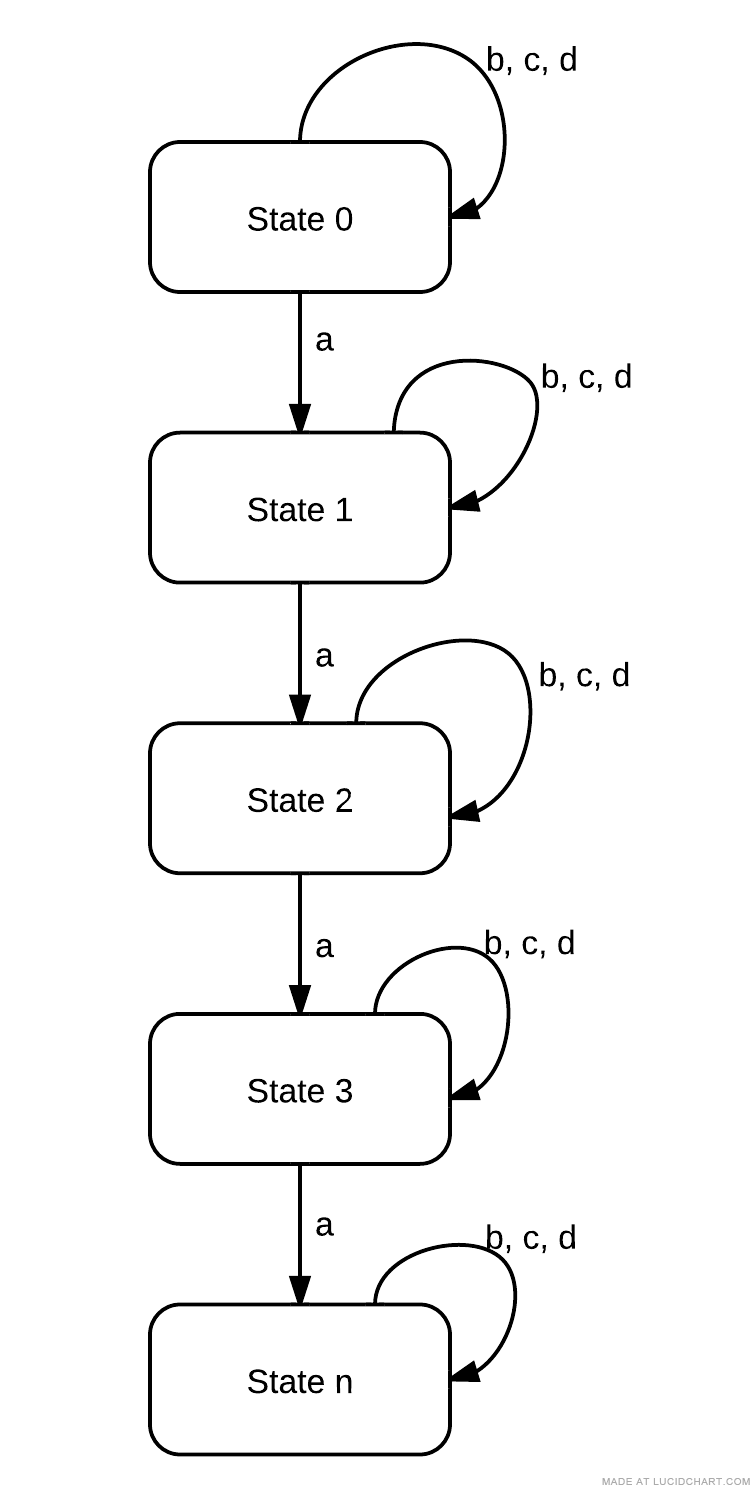
\includegraphics{img/chap6h1.png}}
      \end{center}

      \item The same conditions pertain as in part 1, but the machine
      determines if the sequence contains \emph{at least} three $a$'s.

      \noindent \solution Again $A=\{a,b,c,d\}$. The set of states is
      $\{s_0,s_1,s_2,s_3\}$ where the states have the same meaning
      as before except $s_3$ means we have detected 3 or more $a$'s.
      The next-state function is
      \vspace{5pt}
      \begin{center}
         \begin{tabular}{c|cccc}
	    Present & \\
	    State &   a   &   b   &   c   &   d   \\ \hline
	    $s_0$ & $s_1$ & $s_0$ & $s_0$ & $s_0$ \\
	    $s_1$ & $s_2$ & $s_1$ & $s_1$ & $s_1$ \\
	    $s_2$ & $s_3$ & $s_2$ & $s_2$ & $s_2$ \\
	    $s_3$ & $s_3$ & $s_3$ & $s_3$ & $s_3$ 
	 \end{tabular}
      \end{center}
      \vspace{5pt}
      The state diagram is as follows (with State 3 as the only final
      state).
      \begin{center}
      \scalebox{.2}{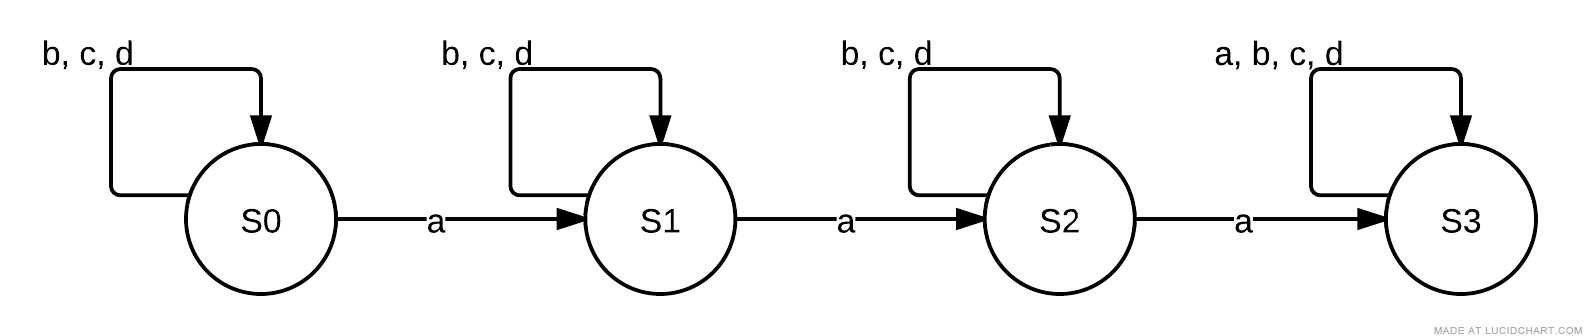
\includegraphics{img/chap6h2.png}}
      \end{center}

      \item The input alphabet consists of the digits 0, 1, 2, 3, 4.
      The machine adds the digits of an input sequence: the addition
      is modulo 5. the sum is to be given by the machine's state
      after the last digit is read.

      \vspace{5pt}
      \noindent \solution $A=\{0,1,2,3,4\}$ and $S=\{s_0,s_1,s_2,s_3,s_4\}$.
      The next-state function is
      \vspace{5pt}
      \begin{center}
         \begin{tabular}{c|ccccc}
	    Present & \\
	    State &   0   &   1   &   2   &   3   &   4   \\ \hline
	    $s_0$ & $s_0$ & $s_1$ & $s_2$ & $s_3$ & $s_4$ \\
	    $s_1$ & $s_1$ & $s_2$ & $s_3$ & $s_4$ & $s_0$ \\
	    $s_2$ & $s_2$ & $s_3$ & $s_4$ & $s_0$ & $s_1$ \\
	    $s_3$ & $s_3$ & $s_4$ & $s_0$ & $s_1$ & $s_2$ \\
	    $s_4$ & $s_4$ & $s_0$ & $s_1$ & $s_2$ & $s_3$
	 \end{tabular}
      \end{center}
      \vspace{5pt}

      The diagram was not done. Trivial.

      \item The machine tells whether or not an incoming sequence of
      0's and 1's ends with 111.

      \noindent \solution $A=\{0,1\}$, $S=\{s_0,s_1,s_2,s_3\}$.
      The next-state function is
      \vspace{5pt}
      \begin{center}
         \begin{tabular}{c|cc}
	    Present & \\
	    State &   0   &   1   \\ \hline
	    $s_0$ & $s_0$ & $s_1$ \\
	    $s_1$ & $s_1$ & $s_2$ \\
	    $s_2$ & $s_2$ & $s_3$ \\
	    $s_3$ & $s_3$ & $s_0$ 
	 \end{tabular}
      \end{center}
      \vspace{5pt}
      The state diagram is as follows (with State 3 as the only final
      state).
      \begin{center}
      \scalebox{.2}{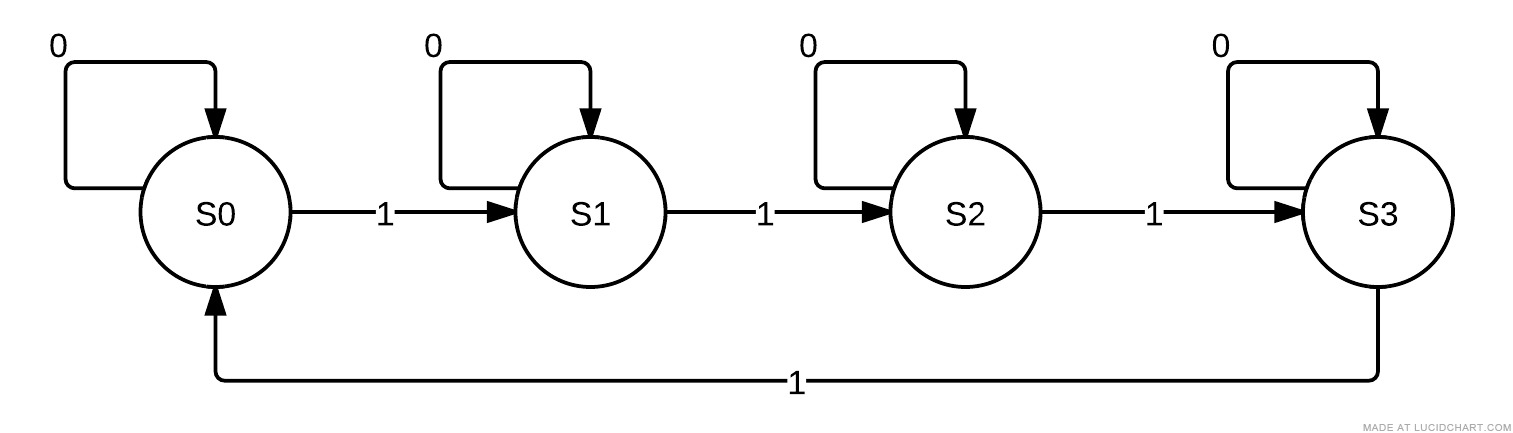
\includegraphics{img/chap6h4.png}}
      \end{center}

      \item If $M$ is a machine whose next-state function is $\alpha$,
      define $\bar{\alpha}$ as follows: If $\textbf{x}$ is an input
      sequence and the machine (in state $s_i$) begins reading
      $\mathbf{x}$, then $\bar{\alpha}(s_i,\mathbf{x})$ is the state of
      the machine after the last symbol of $\mathbf{x}$ is read.
      For instance, if $M_1$ is the machine of the example given above, then 
      $\bar{\alpha}(s_0,11010)=s_1$. (The machine [ed. described in text]
      is in $s_0$ before the first symbol is read; each 1 alters the state,
      but the 0s do not. Thus, after the last 0 is read, the machine is
      in state $s_1$.)

      \begin{enumerate}[(a)]
         \item For the machine $M_1$, give $\bar{\alpha}(s_0,\mathbf{x})$
	 for all three digit sequences $\mathbf{x}$.

         \noindent \solution 
	 \begin{center}
	 \begin{tabular}{cc}
	    $\mathbf{x}$ & $\bar{\alpha}(s_0,\mathbf{x})$ \\ \hline
	             000 & $s_0$ \\
		     001 & $s_1$ \\
		     010 & $s_1$ \\
		     011 & $s_0$ \\
		     100 & $s_1$ \\
		     101 & $s_0$ \\
		     110 & $s_0$ \\
		     111 & $s_1$
	 \end{tabular}
	 \end{center}

	 \item For the machine of part 1, give $\bar{\alpha}(s_i,\mathbf{x})$
	 for each state $s_i$ and every two-letter sequence $\mathbf{x}$.

         \begin{center}
	 \begin{tabular}{c|ccccc}
	    $\mathbf{x}$ & $\bar{\alpha}(s_0,\mathbf{x})$
	       & $\bar{\alpha}(s_1,\mathbf{x})$
	       & $\bar{\alpha}(s_2,\mathbf{x})$
               & $\bar{\alpha}(s_3,\mathbf{x})$
               & $\bar{\alpha}(s_n,\mathbf{x})$\\ \hline
	              aa & $s_2$ & $s_3$ & $s_n$ & $s_n$ & $s_n$ \\
	              ab & $s_1$ & $s_2$ & $s_3$ & $s_n$ & $s_n$ \\
	              ac & $s_1$ & $s_2$ & $s_3$ & $s_n$ & $s_n$ \\
	              ad & $s_1$ & $s_2$ & $s_3$ & $s_n$ & $s_n$ \\
	              ba & $s_1$ & $s_2$ & $s_3$ & $s_n$ & $s_n$ \\
	              bb & $s_0$ & $s_1$ & $s_2$ & $s_3$ & $s_n$ \\
	              bc & $s_0$ & $s_1$ & $s_2$ & $s_3$ & $s_n$ \\
	              bd & $s_0$ & $s_1$ & $s_2$ & $s_3$ & $s_n$ \\
	              ca & $s_1$ & $s_2$ & $s_3$ & $s_n$ & $s_n$ \\
	              cb & $s_0$ & $s_1$ & $s_2$ & $s_3$ & $s_n$ \\
	              cc & $s_0$ & $s_1$ & $s_2$ & $s_3$ & $s_n$ \\
	              cd & $s_0$ & $s_1$ & $s_2$ & $s_3$ & $s_n$ \\
		      da & $s_1$ & $s_2$ & $s_3$ & $s_n$ & $s_n$ \\
		      db & $s_0$ & $s_1$ & $s_2$ & $s_3$ & $s_n$ \\
		      dc & $s_0$ & $s_1$ & $s_2$ & $s_3$ & $s_n$ \\
		      dd & $s_0$ & $s_1$ & $s_2$ & $s_3$ & $s_n$ 
	 \end{tabular}
	 \end{center}

      \end{enumerate}

      \item With each input sequence $\mathbf{x}$ we associate a function 
      $T_x : S \to S$ called a \emph{state transition function}, defined
      as follows:
      \[
         T_x(s_i) = \bar{\alpha}(s_i,\mathbf{x})
      \]

      \noindent For the machine $M_1$ of the example, if $\mathbf{x}=11010$,
      $T_x$ is given by
      \begin{align*}
         T_x(s_0) &= s_1   &   T_x(s_1) &= s_0 
      \end{align*}

      \begin{enumerate}[(a)]
	 \item Describe the transition function $T_x$ for the machine $M_1$ and
	 the following sequences $\mathbf{x}=01001$, $\mathbf{x}=10011$, and
	 $\mathbf{x}=01010$.

	 \noindent \solution 
	 For $\mathbf{x} = 01001$:
	 \begin{align*}
	     T_x(s_0) &= s_0 & T_x(s_1) &= s_1
	 \end{align*}   
	 
	 For $\mathbf{x} = 10011$:
	 \begin{align*}
	     T_x(s_0) &= s_1 & T_x(s_1) &= s_0
	 \end{align*}   

	 For $\mathbf{x} = 01010$:
	 \begin{align*}
	     T_x(s_0) &= s_0 & T_x(s_1) &= s_1
	 \end{align*}   

	 As we can see, $T_x(s_0)=s_0$ when weight of $\mathbf{x}$ is even
	 otherwise $T_x(s_0)=s_1$.

	 \item Explain why $M_1$ has only two \emph{distinct} transition
	 functions. [\textsc{Note}: Two functions $f$ and $g$ are equal
	 if $f(x)=g(x)$ for every $x$; otherwise they are distinct.]
	 
	 \solution As Part 5 implied and we saw in (a) right above here,
	 the defining characteristic of $T_x$ is the weight of $\mathbf{x}$.
	 It is either even or odd. All even weight values of $\mathbf{x}$
	 generate one function, and all odd weight values of $\mathbf{x}$
	 generate another.

	 \item For the machine of part 1, describe the transition function
	 $T_x$ for the following $\mathbf{x}$: $\mathbf{x}=abbca$,
	 $\mathbf{x}=babac$, $\mathbf{x}=ccbaa$.
	 \begin{center}
	 \begin{tabular}{c|ccccc}
	    $\mathbf{x}$ & $T_x(s_0)$ & $T_x(s_1)$ & $T_x(s_2)$ & $T_x(s_3)$
	        & $T_x(s_n)$ \\ \hline
		abbca    & $s_2$ & $s_3$ & $s_n$ & $s_n$ & $s_n$ \\
		babac    & $s_2$ & $s_3$ & $s_n$ & $s_n$ & $s_n$ \\
		ccbaa    & $s_2$ & $s_3$ & $s_n$ & $s_n$ & $s_n$ 
	 \end{tabular}
	 \end{center}

	 \item How many \emph{distinct} transition functions are there
	 for the machine of part 3?

	 \solution The number of distinct machines is 5. The defining 
	 characteristic is the sum of the input sequence $\mathbf{x}$
	 modulo 5. Each sum (0, 1, 2, 3, 4) generates a distinct 
	 transition function. For example, if the sum is 0, then
	 the transition function is the identity function: $T_x(s_i)=s_i$.
	 If the sum is 2, then the transition function is increment by
	 2 (modulo 5): $T_x(s_i) = s_{i+2}$.

      \end{enumerate}

   \end{enumerate}

   \item \textsc{Automata, Semigroups, and Groups}

   By a \emph{semigroup} we mean a set $A$ with an associative operation.
   (There does not need to be an identity element, nor do elements
   necessarily have inverses.) Every group is a semigroup,
   though the converse is clearly false. With every semigroup $A$
   we associate an automaton $M=M(A)$ called the 
   \emph{automaton of the semigroup} $A$. The alphabet of $M$ is $A$,
   the set of states also is $A$, and the next state function is
   $\alpha(s,a)=sa$ [or $\alpha(s,a)=s+a$ if the operation of the semigroup
   is denoted additively].

   \begin{enumerate}[1]
      \item Describe $M(\mathbb{Z}_4)$. That is, give the table of the 
      next-state function, as well as its state diagram.
      
      \solution $A=\{0,1,2,3\}$, $S=\{0,1,2,3\}$. The next-state
      function is:
      \begin{center}
      \begin{tabular}{c|cccc}
          Present \\
	  State &  0  &  1  &  2  &  3 \\ \hline
	    0   &  0  &  1  &  2  &  3 \\
	    1   &  1  &  2  &  3  &  0 \\
	    2   &  2  &  3  &  0  &  1 \\
	    3   &  3  &  0  &  1  &  2
      \end{tabular}
      \end{center}

      The state diagram is:
      \begin{center}
      \scalebox{.2}{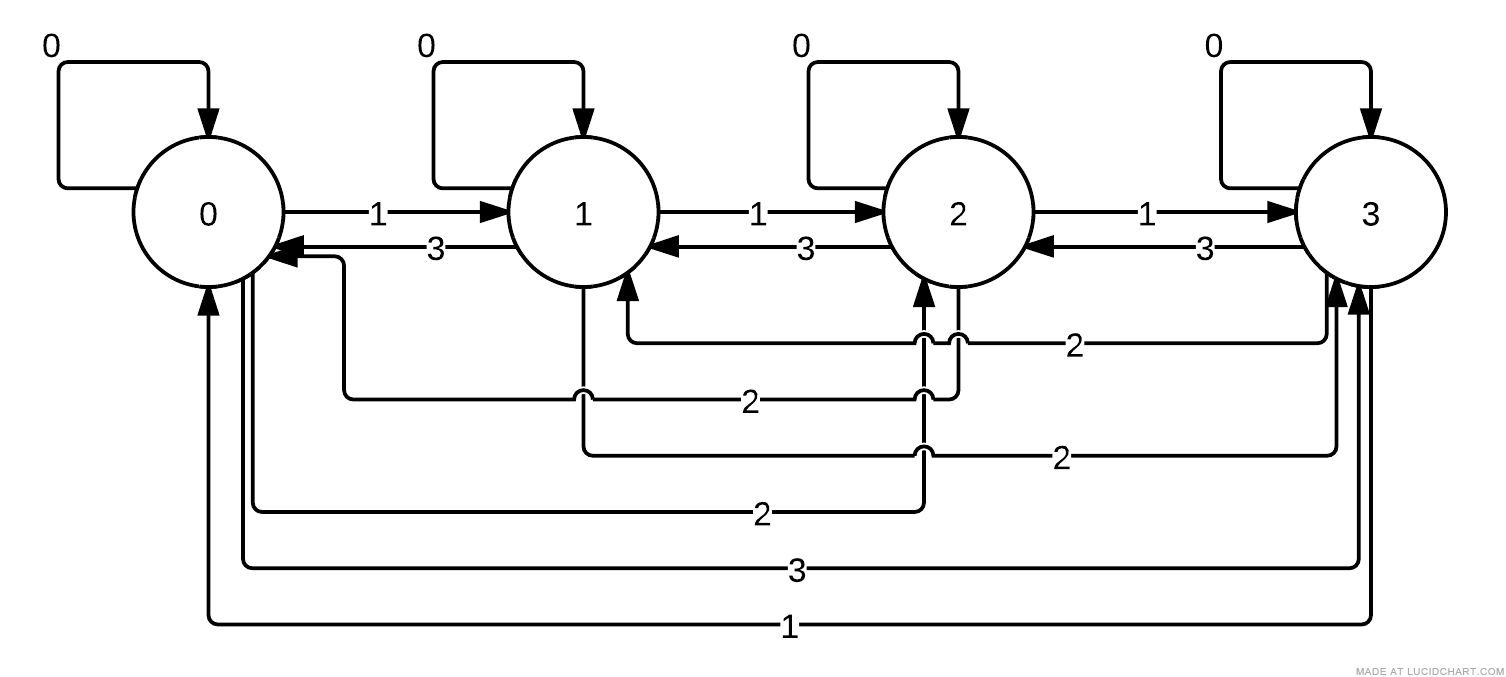
\includegraphics{img/chap6I1.png}}
      \end{center}

      \item Describe $M(S_3)$.

      \noindent \solution I assume $S_3$ is the set $\{s_1,s_2,s_3\}$.
      So $A = S_3$ and $S=S_3$. The next-state function is

      \begin{center}
      \begin{tabular}{c|ccc}
          Present \\
	  State &  $s_1$    &  $s_2$   &  $s_3$ \\ \hline
	 $s_1$  &  $s_1s_1$ & $s_1s_2$ & $s_1s_3$ \\
	 $s_2$  &  $s_2s_1$ & $s_2s_2$ & $s_2s_3$ \\
	 $s_3$  &  $s_3s_1$ & $s_3s_2$ & $s_3s_3$
      \end{tabular}
      \end{center}

      [Update: Chapter 7 finally defines $S_3$. Come back to work on 
      this assignment.]

      \vspace{10pt}
      \hspace{.25in} If $M$ is a machine and $S$ is the set of states of $M$,
      the \emph{state transition functions} of $M$ are functions
      from $S$ to $S$. In the next exercise you will be asked to show
      that $T_y \circ T_x = T_{xy}$; that is, the composite of 
      two transition functions is a transition function. Since the
      composition of functions is associative $[f \circ (g \circ h) =
      (f \circ g) \circ h]$, it follows that the set of all transition
      functions, with the operation $\circ$, is a \emph{semigroup}.
      It is denoted by $\gamma(M)$ [ed. Actually the text uses a
      different symbol but I have no idea what symbol it is so I'm
      using gamma.] and called the \emph{semigroup of the machine} $M$.

      \item Prove that $T_{xy}=T_y \circ T_x$
      \begin{proof}
	  \begin{align*}
             T_{xy} &= \bar{\alpha}(s_i,\mathbf{x}\mathbf{y})\\
	     T_y \circ T_x &= T_y(T_x(s_i)) \\
	                   &= T_y(\bar{\alpha}(s_i,\mathbf{x})) \\
			   &= \bar{\alpha}(\bar{\alpha}(s_i,\mathbf{x}),
			       \mathbf{y}) \\
			   &= \bar{\alpha}(s_i,\mathbf{xy}) 
			       &&\text{Definition of $\bar{\alpha}$}. \qedhere
	  \end{align*}
      \end{proof}

      \item Let $M_1$ be the machine of the example in exercise H above.
      Give the table of the semigroup $\gamma(M_1)$. Does $\gamma(M_1)$
      have an identity element? Is $\gamma(M_1)$ a group?

      \noindent \solution Recall from H5b that $M_1$ has only two distinct
      transtion functions. I will call them $T_0$ for the transition function
      on a sequence with an even number of 1s; and $T_1$ for the transition
      function on a sequence with an odd number of 1s. The table is then

      \begin{center}
      \begin{tabular}{c|cc}
         $\circ$ & $T_0$ & $T_1$ \\ \hline
	   $T_0$ & $T_0$ & $T_1$ \\
	   $T_1$ & $T_1$ & $T_0$ 
      \end{tabular}
      \end{center}

      $T_0$ is the identity element of $\gamma(M_1)$ and 
      $\gamma(M_1)$ is a group as both functions have an inverse:
      $T_0^{-1}=T_0$ and $T_1^{-1}=T_1$.

      \item Let $M_2$ be the machine of Exercise H3. How many \emph{distinct}
      functions are there in $\gamma(M_2)$? Give the table of 
      $\gamma(M_2)$. Is $\gamma(M_2)$ a group? (Why?)

      \solution From H5d we know that there are 5 distinct functions. I
      will call them $T_0, T_1, T_2, T_3, T_4$ where the subscript
      indicates the sum of the sequence modulo 5. The table is then:

      \begin{center}
      \begin{tabular}{c|ccccc}
         $\circ$ & $T_0$ & $T_1$ & $T_2$ & $T_3$ & $T_4$ \\ \hline
	  $T_0$  & $T_0$ & $T_1$ & $T_2$ & $T_3$ & $T_4$ \\
	  $T_1$  & $T_1$ & $T_2$ & $T_3$ & $T_4$ & $T_0$ \\
	  $T_2$  & $T_2$ & $T_3$ & $T_4$ & $T_0$ & $T_1$ \\
	  $T_3$  & $T_3$ & $T_4$ & $T_0$ & $T_1$ & $T_2$ \\
	  $T_4$  & $T_4$ & $T_0$ & $T_1$ & $T_2$ & $T_3$
      \end{tabular}
      \end{center}

      It turns out $\gamma(M_2)$ is a group. The identity element
      is $T_0$. The inverse is given by $T_i^{-1} = T_{0+(-i)}$
      (where the addition in the subscript is obviously modulo 5).

      \item Find the table of $\gamma(M)$ if $M$ is the machine whose
      state diagram is

      \solution The diagram has errors. It is not clear what the
      correct diagram is.
   \end{enumerate}
\end{enumerate}

\end{document}
